\textit{Wireshark}\cite{wireshark} (figura \ref{fig:wire-logo}) es el analizador de tráfico de red más importante y más utilizado. \textit{Wireshark} permite observar el trafico de red en tiempo real y lo muestra en un formato legible para las personas. Cuenta con una gran cantidad de filtros y características, como detectar rápidamente problemas de red como latencia, actividad sospechosa y paquetes caídos. También puede profundizar en el tráfico y descubrir la causa raíz de un problema. Por lo general, los administradores de red usan \textit{Wireshark} para resolver los problemas de latencia causados por los equipos utilizados para enrutar el tráfico alrededor del mundo y para monitorizar los intentos de exfiltración de datos en las operaciones comerciales.\\

\begin{figure}[h]
    \centering
    
\includegraphics[width=0.30\textwidth]{images/sections/tools/wireshark-logo.png}
    \caption{Logo de \textit{Wireshark}}
    \label{fig:wire-logo}
\end{figure}

\textit{Wireshark} consta de un amplio conjunto de funciones que incluye lo siguiente:

\begin{itemize}
    \item Captura en vivo y permite análisis fuera de línea
    \item Análisis completo de \acrshort{voip}
    \item Permite leer/escribir en muchos formatos de archivo de captura diferentes
    \item Captura archivos comprimidos y descomprímalos sobre la marcha
    \item Inspecciona profundamente cientos de protocolos
    \item Utiliza una interfaz de usuario cómoda e intuitiva
    \item Funciona en \textit{Linux}, \textit{Windows}, \textit{Mac OS X} y \textit{FreeBSD}
    \item Tiene potentes filtros de visualización
    \item La salida se puede exportar a \textit{XML}, \textit{CSV}, \textit{PostScript} o como texto sin formato
\end{itemize}

En la siguiente figura (figura \ref{fig:wire-example}), se puede ver un ejemplo de captura de red.

\begin{figure}[h]
    \centering
    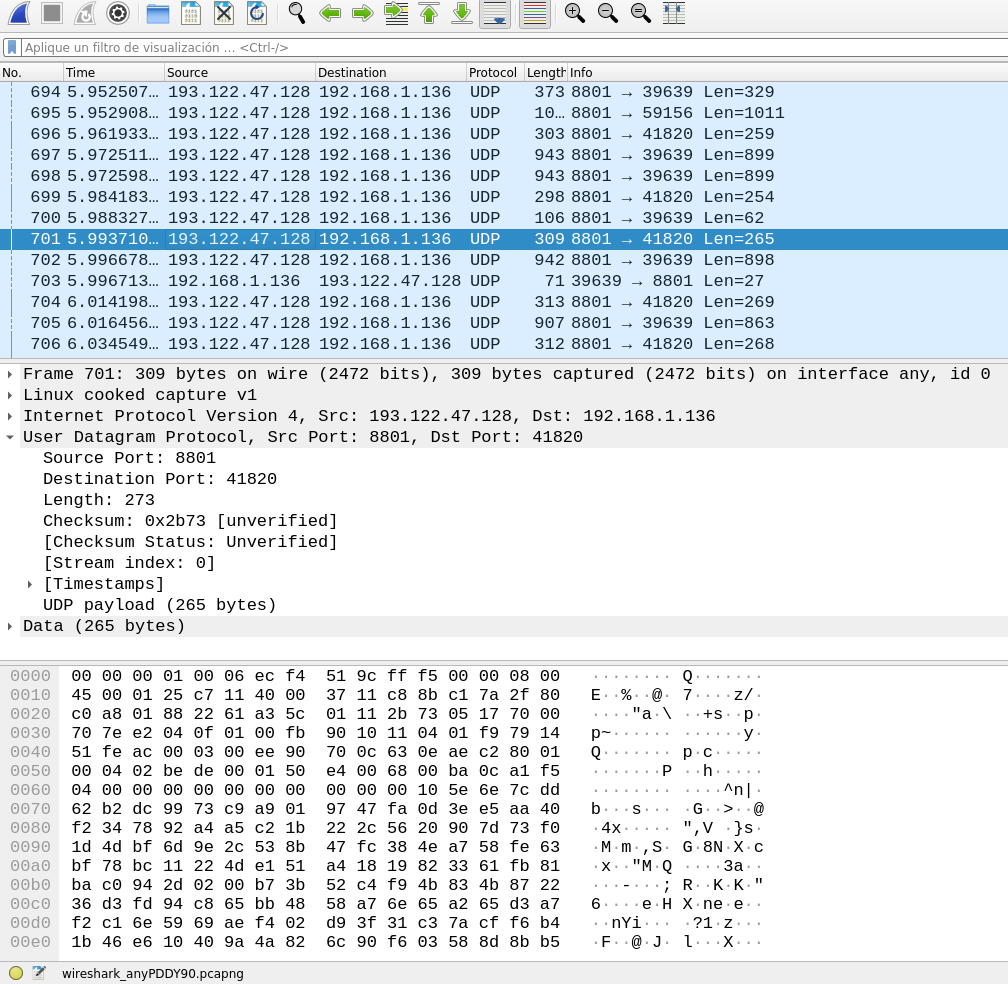
\includegraphics[width=1.0\textwidth]{images/sections/tools/wire-example.png}
    \caption{Captura de red con \textit{Wireshark}}
    \label{fig:wire-example}
\end{figure}